\documentclass[12pt]{article}
%\documentclass{article}
\usepackage{amsmath,amsthm,amssymb}
\usepackage{enumerate}

\usepackage[english]{babel}
 \usepackage{graphicx}
 \usepackage[usenames,dvipsnames,svgnames,table]{xcolor}
\usepackage{palatino}

\usepackage{fancyhdr}
\pagestyle{fancy}
\fancyhf{}
\rhead{Instructor: David Dobor}
\lhead{CIS 2033, Fall 2016, Homework 2}
\rfoot{Page \thepage}


\newenvironment{question}[2][Question]{\begin{trivlist}
\item[\hskip \labelsep {\bfseries #1}\hskip \labelsep {\bfseries #2.}]}{\end{trivlist}}
\newenvironment{answer}[2][Answer]{\begin{trivlist}
\item[\hskip \labelsep {\bfseries #1}\hskip \labelsep {\bfseries #2.}]}{\end{trivlist}}

\begin{document}

\subsection*{\centering{Homework 2}}
\centering\textcolor{blue}{Solutions to Selected Questions. \\}
\centering\textcolor{teal}{\\ ( Homework due in class on Thursday, September 15 )}
\vspace{5mm}


 \begin{question}{1} We roll two fair 6-sided dice. Each one of the 36 possible outcomes is
assumed to be equally likely.
\begin{enumerate}[(a)]
 \item  Find the probability that doubles were rolled.
\item  Given that the roll resulted in a sum of 4 or less, find the conditional probability
that doubles were rolled.
 \item Find the probability that at least one die is a 6.
 \item Given that the two dice land on different numbers, find the conditional probability
that at least one die is a 6.
 \end{enumerate}

\end{question} 

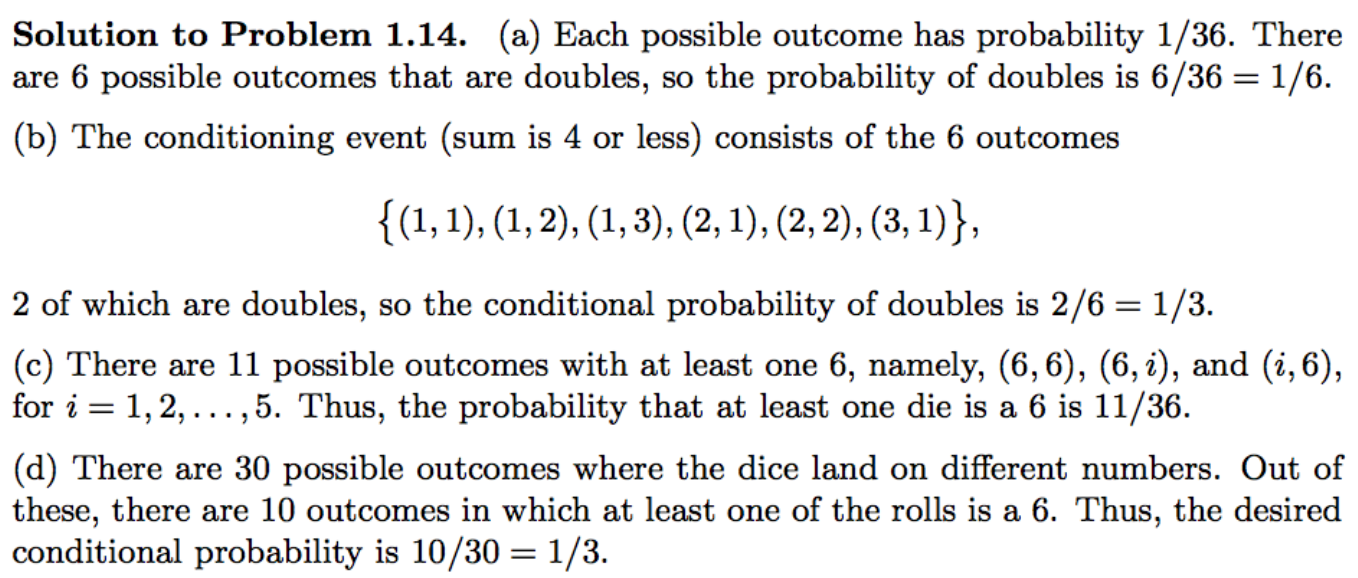
\includegraphics[scale=0.6]{Answer1}

\vspace{5mm}


 \begin{question}{2} A coin is tossed twice. Alice claims that the event of two heads is at least as likely if we know that 
 the first toss is a head than if we know that at least one of the tosses is a head. 
 \begin{enumerate}[(a)]
 \item  Is she right? (try to answer this without peeking into parts (b), (c), and (d) of this question.)
 \item Assume the coin is fair, i.e. all outcomes $\{HH, HT, TH, TT \}$ are equally likely. Let $A$ be the event that the first toss is a head, and $B$ be the event that the second toss is a head. What are - in words - the events $A \cap B$  and "$A \cap B$ given $A$"? Compute $P(A \cap B \mid A)$. 
 \item With the same assumptions and notation as in the previous part, what is the event  "$A \cap B$ given $A \cup B$"? Compute $P(A \cap B \mid A \cup B)$.
 \item Compare the results you got in parts (b) and (c).
 \item  Was Alice right? 
 \item Does it make a difference if the coin is fair or unfair?
 \end{enumerate}
\end{question} 

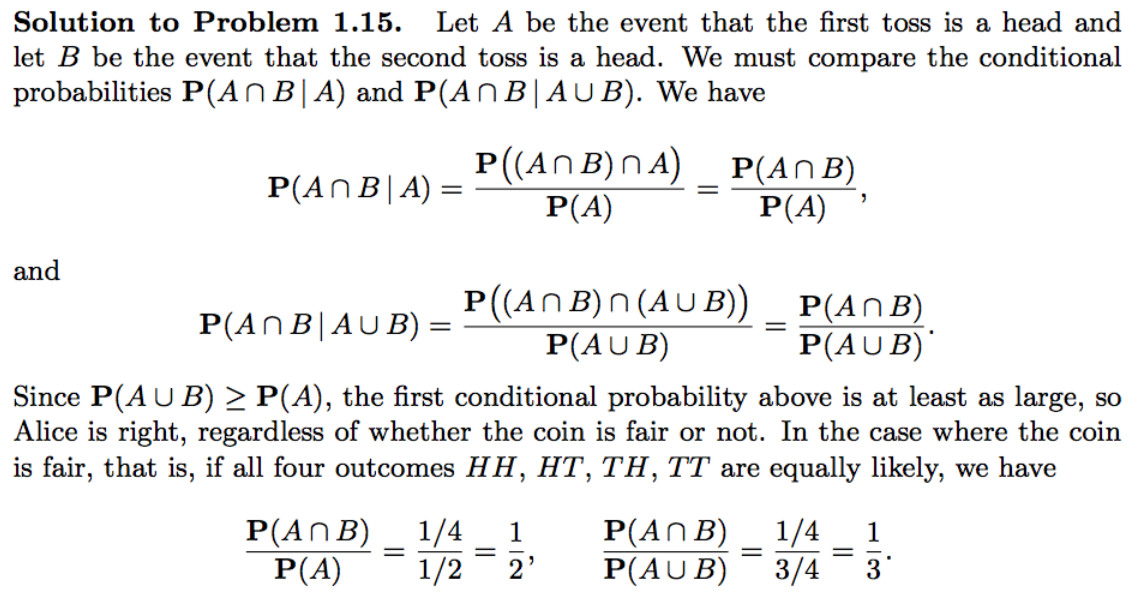
\includegraphics[scale=0.6]{Answer2}
 
\vspace{5mm}

 \begin{question}{3} At a certain stage of a criminal investigation, the inspector in charge is 60
  percent convinced
of the guilt of a certain suspect. Suppose, however, that a \emph{new} piece of evidence
which shows that the criminal has a certain characteristic (such as left-handedness,
baldness, or brown hair) is uncovered. If 20 percent of the population possesses this
characteristic, how certain of the guilt of the suspect should the inspector now be if it
turns out that the suspect has the characteristic?
\end{question} 

 \textbf{\color{TealBlue}\emph{Answer (example 3f, Ross):} }  Letting $G$ denote the event that the suspect is guilty and $C$ the event that he possesses the characteristic of the criminal, we have
  
  \begin{align*}
P(G \mid C) &= \frac{P(G \cap C)} {P(C)}\\
&= \frac{P(C \mid G)P(G)}{P(C \mid G)P(G) + P(C \mid G^c)P(G^c)}\\
&= \frac{1 \times 0.6}{1 \times 0.6 + 0.2 \times 0.4}\\
&\approx .882\\
\end{align*}


\vspace{5mm}
 \begin{question}{4} A ball is drawn at random from an urn containing one red and one white ball. If the white ball is drawn, it is put back into the urn. If the red ball is drawn, it is returned to the urn together with two more red balls. Then a second draw is made. What is the probability a red ball was drawn on both the first and the second draws.
\end{question} 

\end{document}





\begin{align}
&P(A) + P(A^c) + P(B) = P(A \cup A^c \cup B) \\
&P(A) + P(B) \leq 1 \\
&P(A^c) + P(B) \leq 1 \\
&P(A \cup B \cup C) \geq P(A \cup B)
\end{align}


\begin{enumerate}[(a)]
 \item What is $P(Z = 3)$?
\item What is $P(U = 3)$?
 \item What is $P(S \text{ is even })$?
 \end{enumerate}













